\section{Sensor Rig Design}
The sensor rig is designed to carried and operated by a single person, but can also be attached to a vessel.
Two 1m carbon fiber tubes servs as the main structure and provides rigidity to the rig without adding much weight.
Except for the waterproof enclosure and the two carbon fiber tubes, all the mechanical parts are 3D printed, making the sensor rig easy to reproduce and modify.
The various parts are designed to clamp on to the 30mm carbon fiber tubes and friction tape is used to ensure a tight fit.
This makes it easy to extend the rig with additional sensors or design various clamping brackets for attaching the rig to different vessels.
An IP67 rated waterproof enclosure is used to protect the internal electronics from the elements, allowing for operation in all weather conditions.

\begin{figure}[H]
    \centering
    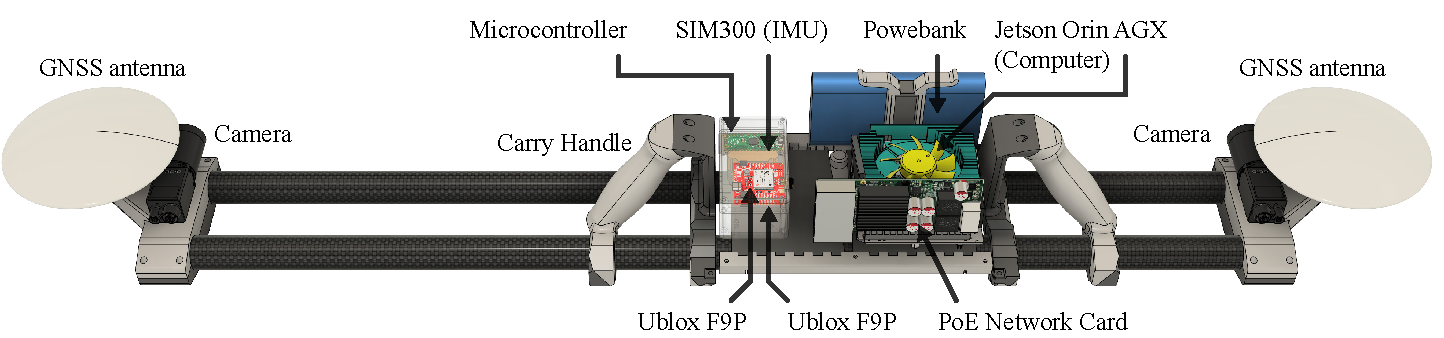
\includegraphics[width=\textwidth]{figures/rig_components.pdf}
    \caption{Cad model of the sensor rig with the enclosure removed for visibility.}
\end{figure}

\subsection{Components}
A camera and a GNSS antenna is mounted on each side of the sensor rig to provide wide baseline stereo video and differential GNSS data for accurate heading estimation.
Inside the waterproof enclosure an Nvidia Jetson Orin AGX serves as the main processing unit.
The Jetson is a single board computer designed for edge computing with a dedicated GPU, GPIO and multiple dedicated hardware for video processing and AI \cite{karumbunathanNVIDIAJetsonAGX2022}.
An external network card is connected to the Jetson through its PCIe slot and provedes 4 separate 1Gb/s ethernet ports with \gls{poe} to power and communicate with the cameras over a single cable.
Two F9P GNSS receivers and a STIM300 \gls{imu} provide the sensor data required for accurate pose estimation.
With a 100wh power bank, the sensor rig can record data for approximately 4 hours before needing a battery change.

\subsection{Control and Monitoring}
The sensor rig hosts a web app that allows the operator to control and monitor the data acquisition from their smartphone.
The web app is built using SvelteKit and TailwindCSS with simplicity in mind, removing the need
From the app the operator can start and stop the aquisition, incoming data from the different sensors and view a live stream from the cameras.
The app also provides information from the Jetson such as CPU temperature, storage usage, \gls{pps} status and battery voltage.
Earlier versions of the app alowed the user to configure parameters such as exposure and gain but we noticed that this took away focus so we swithed to automatic adjustment of these parameters.







